% Directing a multi-machine computation with Claude Code: the method, illustrated by a computation of Choptuik's echo
% period in D dimensions. Build: see Makefile (tectonic). Every number is listed with its source in SOURCES.md.
\documentclass[aps,prd,onecolumn,superscriptaddress,nofootinbib,10pt]{revtex4-2}
\usepackage{amsmath,amssymb}
\usepackage{booktabs}
\usepackage{array}
\usepackage{xurl}
\usepackage{tikz}
\usetikzlibrary{arrows.meta,positioning,calc}
\usepackage{pgfplots}
\pgfplotsset{compat=1.17}
\usepackage[colorlinks=true,linkcolor=blue,citecolor=blue,urlcolor=blue]{hyperref}

\renewcommand{\topfraction}{0.9}
\renewcommand{\bottomfraction}{0.7}
\renewcommand{\textfraction}{0.07}
\renewcommand{\floatpagefraction}{0.8}
\newcolumntype{L}[1]{>{\raggedright\arraybackslash}p{#1}}
\newcommand{\file}[1]{\texttt{#1}}
\newcommand{\prompt}[1]{``\textit{#1}''}

\begin{document}

\title{Directing a multi-machine computation with Claude Code:\\the method behind a computation of Choptuik's echo period}

\author{Nathan Moinvaziri}
\affiliation{Independent researcher}
\date{November 2026; unreviewed draft}

\begin{abstract}
I describe the method by which I carried out a numerical research computation with Claude, Anthropic's model, running in
Claude Code on several machines. The computation is the echo period $\Delta(D)$ of Choptuik's critical solution in $D$
spacetime dimensions, which over 19 days reached down to $D = 3.04375$ and up past $D = 200$. It began in a two-day chat,
which went from a general question to a reproduction of Choptuik's result and then to a search for a formula, before it
moved into a repository and Claude Code. I set the goals, the standards of evidence and the decisions. One coordinating
session wrote all the code and queued numbered tasks. Runner
sessions on the other machines ran the stated commands and reported through an append-only file in the repository, and
the coordinator gave reviews, searches and builds to subagents. I describe the division of roles, the coordination
protocol, how tasks are specified, the rules of evidence and their controls, how runners and subagents were used, and the
patterns that unblocked stuck work, each with a short illustration from the records, and I state the limits of the
approach.
\end{abstract}

\maketitle

\section{Introduction}
\label{sec:intro}

When the collapse of a massless scalar field is tuned to the threshold of black-hole formation, the evolution approaches
a universal solution that repeats itself on ever smaller scales, each echo a copy of the last shrunk by
$e^\Delta$~\cite{Choptuik1993}. The repository \file{choptuik-large-d}~\cite{repo} computes $\Delta$ as a function of the
number $D$ of spacetime dimensions, and its physics is in two companion drafts~\cite{physics,math}. Each point is a
periodic boundary-value problem solved by Newton's method from a prediction made at the last point. At large $D$ the
mass mode amplifies errors at the horizon by a gain $G \approx 0.7^{-(D-3)}$, so the arithmetic must carry more digits as
$D$ grows, from double-double~\cite{Dekker1971} (about 32 digits) through quad-double~\cite{HidaLiBailey2001} (about 64)
to octo-double (about 126). At low $D$ one point costs 4 to 10 hours.

This paper is about the method, not the physics. The project began in a chat on claude.ai (Sec.~\ref{sec:origin}).
Over the following three weeks I directed Claude sessions running in Claude Code~\cite{ClaudeCode} on five machines.
Claude produced the code under my direction. Downward, the lowest converged point is $D = 3.04375$. Upward, a chain of
continuation steps passed $D = 200$ and was still climbing when this was written.

The sources are the chat where the project began~\cite{chat}, the coordination log \file{comms.txt}, the git history, the notes in
\file{notes/}, the raw-data repository~\cite{raw} and the transcripts of the Claude Code sessions on the coordinator
machine. The other machines' side is known from their entries in the log. Every number, quotation and date is listed
with its source in \file{paper/ai/SOURCES.md}.

\section{How it began}
\label{sec:origin}

The chat began with general questions, such as \prompt{Are you able to make new discoveries about physics?} I asked for
\prompt{a toy numerical reality}, and Claude chose a collapse simulation in general
relativity. From 177 runs it reproduced Choptuik's mass scaling, with an exponent of 0.377 and 0.378 for two pulse shapes
against the accepted 0.374, and an echo period $\Delta \approx 3.30$ against 3.445. It named its own limit, a fixed grid
that resolved only about one echo.

The turn came with \prompt{Explain the collapse numbers}. The answer said that both numbers are
eigenvalues of exact problems with no known formula, and it proposed a plan with a literature check first. The check
changed the target, since a 2026 paper had already computed $\Delta$ for continuous $D$ between 3.05 and 5.5
(see~\cite{physics}).
Claude then computed the critical solution directly, as a periodic problem rather than a simulation. At 63 Fourier modes
it gave $\Delta = 3.4454523972$ in four dimensions, which agrees with the best published value, $3.445452402$, to nine
digits, and it went on to scan $D$.

Four prompts then pushed toward a formula: \prompt{Yes continue to find the formula you are doing great don't give up.
It exists}, \prompt{Could it be a sum?}, \prompt{What if is a combination of a small sum and large sum?} and
\prompt{Where is the formula?} They shaped the method in two ways. First, each suggested form
was turned into a fit and tested on dimensions it had not seen, as when a fit to $D \le 8$ predicted the computed values
out to $D = 10.1$ to within $2\times10^{-5}$. That habit later became the held-out and planted-truth tests of
Sec.~\ref{sec:evidence}. Second, the search produced a structural finding. The solutions that compete with the smooth one
behave like $(1-x)^s$ near the horizon, with $s$ measured to grow like $0.6\,(D-2)$, so the condition that fixes $\Delta$
weakens rapidly with $D$ and no plain series in $1/D$ can fix it. Claude called the expected form a transseries, and the
idea became Proposition 1 of the later work, ``the $1/n$ expansion never fixes the period''. The fitted formulas
themselves did not last. The first one for $\Delta$, fitted on data below $D = 11$, fell like $(D-2)^{-1/4}$, while the
later data give a finite limit, $\Delta_\infty = 1.643893746$~\cite{physics}.

A formula needed many precise points, so speed became the problem. I asked \prompt{can we speed up the runtime by using
SIMD?} and \prompt{Does it make sense to rewrite in Rust?}, and then \prompt{With a subagent make a purpose build Rust
build and measure speed.}, the first subagent of the project. The chat ran in a cloud container with two virtual cores.
I put what the chat had produced into a repository, whose first commit is ``Import the DSS residual kernel'', and linked
the chat to my laptop: \prompt{You are now local on my computer. It has AVX512 too which is nice. Continue our work.}
Within hours the first entries of \file{comms.txt} passed between a cloud session and the laptop, and the method of the
following sections grew from that pair.

\section{Roles}
\label{sec:roles}

\emph{I} set the goals, from \prompt{continue to D = 200} to \prompt{we can push past D=200 and go as large as we
can}. I set the standards of evidence and chose between options, by short prompts and by answering
the coordinator's multiple-choice questions. I also acted on the machines myself. I merged and released the arithmetic
library \file{multidouble}~\cite{multidouble}, and I woke, plugged in and set up machines.

\emph{The coordinator} was one Claude Code session at a time, first on a cloud machine and then on the Mac. It wrote all the code in its own worktrees, merged results into main, wrote the notes and queued numbered tasks, T1
to T135.

\emph{The runners} were one Claude Code session per other machine. They ran the commands of their tasks, posted results
and pushed raw output, and they did not edit code. That rule came from my prompt \prompt{make a note that
the other machines are running a lower model than you are, so it is best for you to write any code and not them.} The Mac
runner's transcripts record Claude Sonnet 5.5 from then on.

\emph{Subagents} were sessions the coordinator started for one bounded task, each returning a single report.

\begin{table}[h]
\caption{The machines, by their names in \file{comms.txt}, with the entries each posted (headers counted at commit
07eff89). The laptop posted as \file{local} at first.}
\label{tab:machines}
\small
\begin{tabular}{L{1.4cm}L{5.4cm}L{7.4cm}r}
\toprule
name & machine & role & entries\\
\midrule
\file{cloud} & cloud container, 2 cores, 6.27 GB & coordinator to 26 October; then the coordinator's name on the Mac & 293\\
\file{win} & Windows laptop, 4 cores and 8 threads, 31.8 GB & runner from 19 October: low $D$, builds, second paths & 318\\
\file{mac} & Mac, Apple M5, 10 cores & runner from 24 October to 5 November; coordinator from 26 October & 221\\
\file{win2} & Windows desktop, 20 cores, 95.6 GB & runner from 1 November: the large-$D$ chain, low-$D$ legs & 134\\
\file{macm3} & Mac laptop, Apple M3, 8 cores, 24 GB & runner from 6 November: a second path past $D = 193.77$ & 8\\
\bottomrule
\end{tabular}
\end{table}

\begin{figure}[t]
\centering
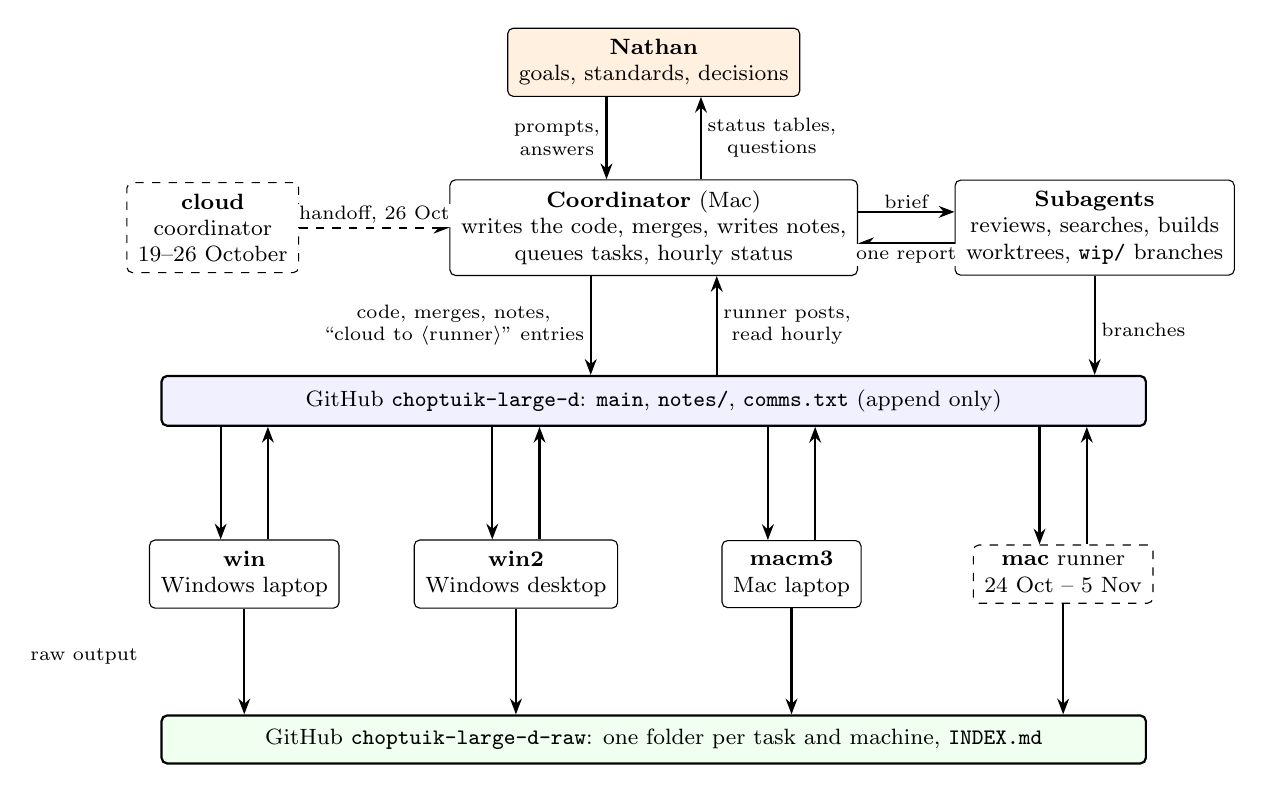
\begin{tikzpicture}[
  box/.style={draw, rounded corners=2pt, align=center, font=\footnotesize, inner sep=4pt, fill=white},
  hub/.style={draw, thick, rounded corners=2pt, align=center, font=\footnotesize, inner sep=5pt, fill=blue!6},
  lab/.style={font=\scriptsize, align=center, fill=white, inner sep=1pt},
  arr/.style={-{Stealth[length=2mm]}, thick},
  darr/.style={-{Stealth[length=2mm]}, thick, dashed}]
\node[box, fill=orange!12] (me) at (0,5.2) {\textbf{Nathan}\\goals, standards, decisions};
\node[box] (coord) at (0,3.1) {\textbf{Coordinator} (Mac)\\writes the code, merges, writes notes,\\queues tasks, hourly status};
\node[box, dashed] (cloud) at (-5.6,3.1) {\textbf{cloud}\\coordinator\\19--26 October};
\node[box] (sub) at (5.6,3.1) {\textbf{Subagents}\\reviews, searches, builds\\worktrees, \texttt{wip/} branches};
\node[hub, minimum width=12.5cm] (main) at (0,0.9) {GitHub \texttt{choptuik-large-d}: \texttt{main}, \texttt{notes/}, \texttt{comms.txt} (append only)};
\node[box] (win) at (-5.2,-1.3) {\textbf{win}\\Windows laptop};
\node[box] (win2) at (-1.75,-1.3) {\textbf{win2}\\Windows desktop};
\node[box] (m3) at (1.75,-1.3) {\textbf{macm3}\\Mac laptop};
\node[box, dashed] (macr) at (5.2,-1.3) {\textbf{mac} runner\\24 Oct -- 5 Nov};
\node[hub, minimum width=12.5cm, fill=green!6] (raw) at (0,-3.4) {GitHub \texttt{choptuik-large-d-raw}: one folder per task and machine, \texttt{INDEX.md}};
\draw[arr] ([xshift=-6mm]me.south) -- node[lab, left=1pt] {prompts,\\answers} ([xshift=-6mm]coord.north);
\draw[arr] ([xshift=6mm]coord.north) -- node[lab, right=1pt] {status tables,\\questions} ([xshift=6mm]me.south);
\draw[darr] (cloud.east) -- node[lab, above] {handoff, 26 Oct} (coord.west);
\draw[arr] ([yshift=2mm]coord.east) -- node[lab, above] {brief} ([yshift=2mm]sub.west);
\draw[arr] ([yshift=-2mm]sub.west) -- node[lab, below] {one report} ([yshift=-2mm]coord.east);
\draw[arr] ([xshift=-8mm]coord.south) -- node[lab, left=1pt] {code, merges, notes,\\``cloud to $\langle$runner$\rangle$'' entries} ([xshift=-8mm]main.north);
\draw[arr] ([xshift=8mm]main.north) -- node[lab, right=1pt] {runner posts,\\read hourly} ([xshift=8mm]coord.south);
\foreach \r in {win, win2, m3, macr} {
  \draw[arr] ([xshift=-3mm]main.south -| \r.north) -- ([xshift=-3mm]\r.north);
  \draw[arr] ([xshift=3mm]\r.north) -- ([xshift=3mm]main.south -| \r.north);
  \draw[arr] (\r.south) -- (raw.north -| \r.south);
}
\node[lab, anchor=east] at ([xshift=-1mm]win.west |- 0,-2.35) {raw output};
\draw[arr] (sub.south) -- node[lab, right=1pt, pos=0.55] {branches} (sub.south |- main.north);
\end{tikzpicture}
\caption{The participants and how they were connected. I spoke only to the coordinator, and the coordinator spoke to the
runners only through \file{comms.txt}. Each runner's watcher wakes it when an entry addressed to it arrives (down arrows),
its posts carry its processor and memory use (up arrows), and its raw output goes to the raw-data repository. Dashed boxes
are sessions that ended.}
\label{fig:arch}
\end{figure}

\section{The coordination protocol}
\label{sec:protocol}

\emph{One log.} All sessions talked through \file{comms.txt} in the code repository (Fig.~\ref{fig:arch}). It is
append-only. Each entry has a header such as \file{== 2026-11-06 13:34 UTC cloud to win2}, with the time read from a
clock, and a writer pulls, appends, commits only that file and pushes. It held 974 entries when this was written.
When the coordinator moved to the Mac, I chose to keep \file{cloud} as its name so the runners' watchers needed no
change.

\emph{Watchers.} A runner waits with \file{comms\_watch.py}, which fetches the repository every 60 s and exits when an entry
addressed to its name arrives, waking the session. After 110 minutes it exits anyway, because Claude Code stops a
background command after two hours, and the session restarts it. It costs nothing while it waits, and it replaced
polling loops.

\emph{Raw output} goes to a separate repository, one folder per task and machine, each with a README whose first line
says what it holds, indexed by \file{INDEX.md}. The long-running scripts refuse any other output path, and
\file{raw\_check.py} fails when a folder a post names is not on GitHub. The rule followed a loss. Early on the
coordinator found that the per-point records of 757 early points had stayed on the cloud machine's disk and were gone,
though their values survived. I then asked \prompt{from now on all agents should store the raw output in git somewhere
different.}

\emph{Status.} A recurring prompt asked the coordinator every hour to fetch, read the new entries, check the branches and
report. It fired 308 times. I shaped the answer into one table row per runner and task, naming the problem each task
serves and an ETA in hours, and I asked the runners to report processor and memory use so idle capacity would show.

\section{How a task is specified}
\label{sec:tasks}

A task entry states its commands, its thread count, its stop conditions and what to push (AGENTS.md). A shortened
example, the entry that sent the octo-double chain to win2, shows the form.
{\footnotesize
\begin{verbatim}
1. win2, T129 (the chain to 200 in octo-double): ... below normal, 18 threads:
     anm_run.py ..\..\choptuik-large-d-raw ..\..\choptuik-large-d-raw\T129-win2\chain
       --state T127-win2/chain2/anm_pin3_D175.5246.npz --kfreeze 3 --N 24 ... --jet_o 1
   ... Stop at D_max, on a degenerate series, when two steps in a row need a of 0.125
   or less, or after 10 h. Push T129-win2/ at each post.
\end{verbatim}
}
\noindent Four further habits made tasks robust.
\begin{itemize}
\item \emph{Pilots first.} A long run starts with a short run of its hardest case and a written stop condition. The switch
of the chain to octo-double followed a two-step pilot run beside the old chain.
\item \emph{Rules the runner applies without waiting.} An entry can arm a rule, such as ``if the log gains no line for 20
minutes while one core is busy, take one py-spy dump, kill the tree, restart from the last state with h\_max halved (0.25,
then 0.125), and post. Do not wait for me.'' Another told win2 to ``Switch it yourself, without waiting for me, when an
accepted stall passes 1e-26, or when chain4 stops on three halvings''.
\item \emph{Second paths.} A new value counts once another run, usually on another machine, reaches the same $D$. On the
chain, 18 such runs give the error column of 66 rows, with differences from $1.9\times10^{-32}$ to $2.9\times10^{-19}$.
\item \emph{Reporting, not fixing.} A runner that sees a mismatch posts it and continues or waits as the task says. ``Do not
edit code; on an error, stop and post it'' closes eleven entries.
\end{itemize}

\section{Rules of evidence}
\label{sec:evidence}

AGENTS.md states the rules, partly taken from the verification protocols of
BootLoops~\cite{BootLoops}. Every check must be able to fail, so each check is broken once on purpose and the broken
version stays runnable. Planted truth comes before real data. Every error bar says what it is. Independent checks share
none of the machinery under test. Discrepancies are reported, not quietly fixed, and thresholds are not loosened to pass.
Every quoted number is tied to a file by \file{check\_numbers.py}, which also checks that each test rejects a value
shifted by one unit. Table~\ref{tab:checks} shows the rules in the late large-$D$ work.

\begin{table}[h]
\caption{Checks and their controls in the late large-$D$ and low-$D$ work. Each control was run and failed as it must.}
\label{tab:checks}
\small
\begin{tabular}{L{4.2cm}L{4.1cm}L{4.4cm}L{2.8cm}}
\toprule
check & pass & control, which must fail & source\\
\midrule
re-seed of a stored prediction (\file{checkq}) & converges, $2.25\times10^{-37}$ at 153.43 & the previous rule stops at $3.60\times10^{-23}$, exit 1 & QUAD\_DOUBLE 13.26--27\\
bit identity of a new build & 28 of 28 jet outputs equal & a mutated constant, 28 of 28 differ & OCTO\_DOUBLE 3\\
octo-double series against two quad-double forms & within 30 times their spread at every order & the double-double series, off by up to $10^{25}$ & OCTO\_DOUBLE 3\\
octo-double corrector from a planted start & $6.86\times10^{-42}$, $\Delta$ to $1.18\times10^{-34}$ & one term through the quad-double LU, stops at $3.39\times10^{-12}$ & OCTO\_DOUBLE 5.4\\
every value of $\Delta$ against its source & 2445 rows equal & one row moved by one ulp, exit 1 & QUAD\_DOUBLE 13.25\\
low-$D$ planner probe, smoke test & every case plans, exit 0 & a cap of 0.001 s caps all, exit 1 & LOW\_D 16\\
\bottomrule
\end{tabular}
\end{table}

A control that does not fire leaves its check untested. That happened once, in the octo-double kernel's tests, where a
planted change landed in a part that quad-double still holds. The planted root was moved and the criteria were kept.

\section{Runners and subagents}
\label{sec:agents}

\emph{Runners} built the solver and checked each build bit for bit against stored references, ran the chains and the
low-$D$ legs, and posted per-step numbers. Their value lay as much in what they flagged. Table~\ref{tab:patterns} lists
the failure modes the records show, with an example and the remedy that followed. The coordinator's own errors appear
there too. Of the fifteen coordinator errors the records show, eight were caught by another Claude session, five by the
coordinator's own checks and two by me.

\begin{table}[t]
\caption{Failure modes of the multi-session setup, with examples from \file{comms.txt} and the remedy adopted.}
\label{tab:patterns}
\small
\begin{tabular}{L{3.0cm}L{8.0cm}L{5.0cm}}
\toprule
failure mode & example & remedy\\
\midrule
a command that does not run as written & a relaunch of a stopped run exited at once (T82); a check's arguments were wrong (T126, T133). The runner found the cause in the code and said what it did instead. & a correction entry; runners describe any deviation\\
a wrong expectation in the task & a control expected to fail one check failed three (T104b); a check compared a computed plan across operating systems (T112). The runner reported and did not fix. & the coordinator corrects its text or the check\\
a cause misread & win2 read re-seed failures as a platform difference (T118, T127); the coordinator replayed the stored inputs and found the code & store every input a failure depends on\\
a timing rule that misfires & a 30-minute hang rule shorter than one 31-minute series (macm3); a slow LU read as stuck after 3.7 h (T132); a sleeping Mac read as oversubscribed & rules tied to processor use; phase timers; a stack dump before a kill\\
a watcher that stops & Claude Code stopped the laptop's watcher under memory pressure, once for 56 hours that the status missed, until I asked \prompt{the win machine is not doing anything?} & silence shown in the status; restart on the author's word in that session\\
a machine that sleeps & the Mac hibernated for 7 hours, and once ran out of battery; the laptop slept on battery & \file{caffeinate} tied to runs; awake-time accounting; an always-on desktop (win2)\\
\bottomrule
\end{tabular}
\end{table}

One lesson about authority came from the watcher. When I asked the coordinator to tell the laptop to restart its own
watcher after a build, the instruction relayed through the log did not count as mine, and the laptop's session restarted
it only when I asked in that session.

\emph{Subagents.} The coordinator's transcript records 29 subagent launches for this project. Six were reviews and audits,
among them the readability of the papers, the README and the quoted numbers (17 findings, 13 fixed). Six were searches,
such as methods for continuing to large $D$. Six were analyses, such as the low-$D$ code and a formula for $\Delta(D)$.
Ten were builds, among them pull requests to \file{multidouble}, re-seeding of the horizon data and the octo-double
corrector, and one wrote this paper. The coordinator used them where independence mattered (a reviewer that did not write
the work), where a wide search would fill its own context, and where a build of hours could run beside its work. My
standing instruction is not to use subagents without asking and naming their number, and 26 of the 29 followed a prompt
of mine asking for one, such as \prompt{run two subagents if u need to}. From the third week on, every brief named a git
worktree and many a backup branch \file{wip/$\langle$topic$\rangle$}. The coordinator checked each report before relaying it. When
it merged the octo-double series, its smoke test showed that the merged driver imported the new helpers at module level,
which would have broken every other path on the runners' older packages, and it moved the import. A subagent's code
analysis also corrected one of the coordinator's diagnoses, a stall at low $D$ that was in fact a stale checkpoint.

\section{Unblocking stuck work}
\label{sec:unblock}

The large-$D$ chain met five walls in its last day (Fig.~\ref{fig:frontier}). Each was passed by one of a few patterns.

\begin{figure}[t]
\centering
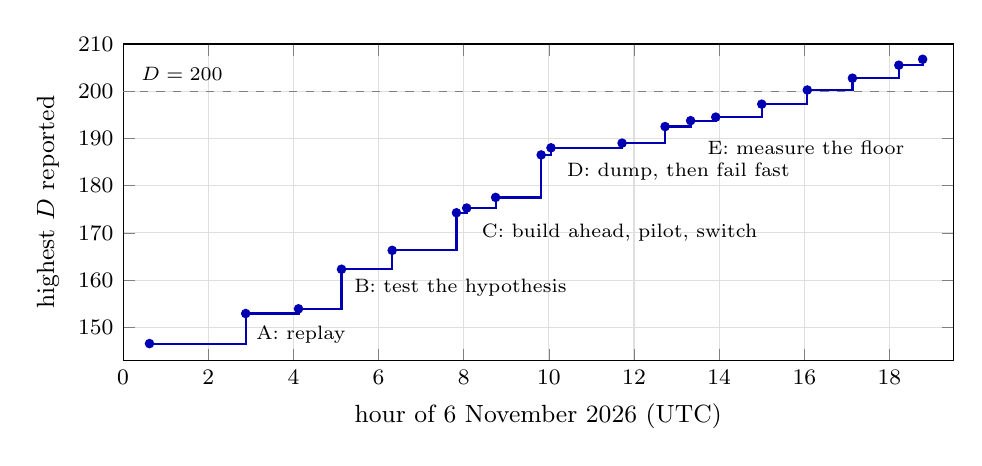
\begin{tikzpicture}
\begin{axis}[width=\textwidth, height=5.6cm, xmin=0, xmax=19.5, ymin=143, ymax=210,
  xlabel={hour of 6 November 2026 (UTC)}, ylabel={highest $D$ reported},
  xtick={0,2,...,18}, ytick={150,160,...,210}, grid=major, grid style={gray!25},
  tick label style={font=\footnotesize}, label style={font=\small}]
\addplot[const plot, thick, blue!70!black, mark=*, mark size=1.3pt] coordinates {
 (0.62,146.56) (2.88,152.93) (4.12,153.93) (5.13,162.31) (6.32,166.31) (7.83,174.27) (8.07,175.27)
 (8.75,177.52) (9.82,186.52) (10.05,188.02) (11.72,189.02) (12.73,192.52) (13.33,193.77) (13.92,194.52)
 (15.00,197.27) (16.07,200.27) (17.13,202.77) (18.22,205.52) (18.78,206.77)};
\draw[dashed, gray] (axis cs:0,200) -- (axis cs:19.5,200);
\node[font=\scriptsize, align=left, anchor=west] at (axis cs:2.9,148.5) {A: replay};
\node[font=\scriptsize, align=left, anchor=west] at (axis cs:5.2,158.5) {B: test the hypothesis};
\node[font=\scriptsize, align=left, anchor=west] at (axis cs:8.2,170.0) {C: build ahead, pilot, switch};
\node[font=\scriptsize, align=left, anchor=west] at (axis cs:10.2,183.0) {D: dump, then fail fast};
\node[font=\scriptsize, align=left, anchor=west] at (axis cs:13.5,188.0) {E: measure the floor};
\node[font=\scriptsize, anchor=south west] at (axis cs:0.2,200.3) {$D = 200$};
\end{axis}
\end{tikzpicture}
\caption{The highest $D$ in the runners' posts on 6 November, with the walls at 152.93, 162.31, about 171, 188.02 and
193.77, labelled by the pattern of Sec.~\ref{sec:unblock} that passed each. The chain ran on win2, and the fixes were made
on the Mac.}
\label{fig:frontier}
\end{figure}

\emph{A. Replay the failure on its stored input.} At 152.93 every re-seed of the horizon data failed. Twenty-two minutes
after the stop I wrote \prompt{we need to keep going above 150}, and the coordinator replayed the failing step on the Mac
instead of waiting for a queued replay. Within 34 minutes it had found two defects, a polish that gave up after six steps
and a corrector that stored an unprojected state, and fixed both with a control that fails on the old rule. From then on
the runs saved their predictions, so later failures could be replayed offline on the real case.

\emph{B. Test the hypothesis before acting on it.} At 162.31 the coordinator's first reading was an imprecise Jacobian,
which would have made the coming octo-double series useless there. A cheap test showed the quad-double and octo-double
Jacobians equal to $1.2\times10^{-36}$, and the stored predictions then let candidate rules be compared on the failing
input until one converged (\file{notes/QUAD\_DOUBLE.md} 13.27).

\emph{C. Build the next precision ahead of need, pilot it, then switch.} I wrote \prompt{yes add octo-double
jets in hp engine, we don't need to run it until it is needed.} When a runner flagged the quad-double series losing
digits near 171, a two-step pilot showed the octo-double series healthy and $\Delta$ unchanged in 21 printed digits, and
the switch took one entry. The octo-double corrector followed the same path. It was built by a subagent with a planted
check and a failing control, merged at c496ac8 (\file{notes/OCTO\_DOUBLE.md} 5--6), and handed to the
runners as a rule to switch on their own.

\emph{D. Dump the stack before killing, then fail fast.} Above 188.02 a step ran on one core for more than an hour with
no output.
The runner did not kill it but asked, the coordinator asked for a py-spy~\cite{pyspy} dump first, and the dump put the
hang somewhere other than where the coordinator had guessed. A fail-fast on that path and an armed hang rule followed.

\emph{E. Measure the floor and accept it explicitly.} At 193.77 the quad-double corrector stalled at $1.0$ to
$1.1\times10^{-28}$ against its tolerance of $10^{-28}$, and halving could not help. After my prompt \prompt{we can push
past D=200 and go as large as we can}, the coordinator measured the floor on stored states and added a rule that accepts
a stall below $10^{-24}$, with a flag at $10^{-26}$ and a second path on macm3. This rule weakens the convergence test,
and I record it as such. Its measured effect on $\Delta$ is $2\times10^{-18}$ to $1.1\times10^{-17}$ so far, and the
runners switch to the octo-double corrector when the flag fires.

\emph{F. Planted truth for a diagnostic.} At low $D$ the planner froze at $D = 3.04375$. Before reading the probe that
separates a bad prediction from a bad planner, its procedure fixed a planted case that must reproduce the known freeze and
a control that must fail (\file{notes/LOW\_D.md} 16). The same episode shows the cost of a wrong rule. The coordinator
told the laptop that no output after 3.7 hours meant stuck, the laptop's dump showed a slow LU instead, and the probe now
times each phase. That question was still open at the time of writing.

Table~\ref{tab:prompts} lists the prompts of mine that moved stalled work, from the chat of Sec.~\ref{sec:origin} on.
Most were short. Their effect was to replace deliberation by an action, to remove a limit that the work had taken for
granted, or, in the chat, to keep a search going and suggest a form to test.

\begin{table}[t]
\caption{Prompts that moved stalled work, verbatim, and what followed.}
\label{tab:prompts}
\small
\begin{tabular}{L{1.8cm}L{5.4cm}L{8.8cm}}
\toprule
when & prompt & what followed\\
\midrule
18 Oct 16:43 & \prompt{Explain the collapse numbers} & A reproduction became a direct computation, checked against the literature, then a scan in $D$.\\
18 Oct 20:41 & \prompt{Could it be a sum?} & Suggested forms were fitted and tested on unseen $D$, and the search found why no plain $1/D$ series fixes $\Delta$.\\
27 Oct 06:56 & \prompt{just make the quad-double solver, stop delaying.} & The quad-double solver was built that morning, with precision tests.\\
2 Nov 22:40 & \prompt{just jump to 100} & Jumps of every size failed past 79.3, which located the wall in Newton's basin rather than the step rule.\\
3 Nov 19:21 & \prompt{have a subagent scourer the internet and scientific papers for ways continue large D} & A literature subagent found high-order Taylor continuation in $D$~\cite{Cochelin1994}, which became the chain.\\
5 Nov 02:34 & \prompt{have a subagent build the real thing and not a toy.} & Re-seeding of the horizon data moved from a model into the real solver.\\
5 Nov 22:25 & \prompt{yes add octo-double jets in hp engine, we don't need to run it until it is needed.} & The octo-double series was ready before the quad-double one failed (pattern C).\\
6 Nov 03:15 & \prompt{we need to keep going above 150} & Immediate replay and fix of the stall at 152.93 (pattern A).\\
6 Nov 13:28 & \prompt{we can push past D=200 and go as large as we can} & The chain's limit went to 1000 with an explicit stall rule (pattern E).\\
6 Nov 13:54 & \prompt{can we queue it on a machine that is not busy?} & The low-$D$ probe moved to the laptop, displacing a lower-value task.\\
6 Nov 14:25 & \prompt{i can spool up another mac M3 laptop if you think it will help make the total work faster.} & macm3 was set up and bit for bit with the Mac's build in 75 minutes, then ran a second path.\\
\bottomrule
\end{tabular}
\end{table}

\section{The records}
\label{sec:numbers}

Table~\ref{tab:numbers} counts the records the method left. The log, the commits and the raw-data folders together let a
result be traced from its entry to its run and its output.

\begin{table}[h]
\caption{The records, at commit 07eff89 of the code repository and d0f3311 of the raw-data repository.}
\label{tab:numbers}
\small
\begin{tabular}{L{5.2cm}L{10.6cm}}
\toprule
quantity & value\\
\midrule
chat on claude.ai & 17 October, 23:24, to 19 October, 06:18; 62 prompts, a few on side projects\\
period of the repository & 19 October 2026, 03:53, to 6 November, 18:26; 19 days\\
commits on main & 2227, of which 954 are entries of \file{comms.txt}\\
entries in \file{comms.txt} & 974: coordinator 293, Windows laptop 318, Mac 221, Windows desktop 134, macm3 8\\
tasks & T1 to T135\\
raw-data repository & 124 folders (laptop 61, Mac 44, desktop 17, macm3 2), 548 commits\\
values of $\Delta$ in \file{hp/data/delta\_all.csv} & 2445 rows, from $D = 3.04375$ to 203.27\\
coordinator session on the Mac & 334 prompts, 308 hourly status prompts, 29 context summaries, 30 subagent launches\\
\bottomrule
\end{tabular}
\end{table}

\section{Limitations and lessons}
\label{sec:limits}

\emph{No expert has reviewed the work.} I have not checked the mathematics myself. The checks of Sec.~\ref{sec:evidence}
make the work testable, and they do not replace a reviewer.

\emph{The records are incomplete.} The cloud sessions of the first week left no transcript on the coordinator machine,
and the runners' transcripts stayed on their machines. The per-point records of 757 early points are lost.

\emph{The error bars are of several kinds.} Differences between runs measure the path dependence of the held harmonics,
about $10^{-20}$, and the stall rule, $10^{-18}$ to $10^{-17}$. Neither includes the bias of the held harmonics, $10^{-8}$ to
$10^{-7}$ at $D = 79$ to 86, which the README states separately.

\emph{Wrong instructions cost the most.} The runners carried out tasks as written, so a wrong rule cost what it said.
What corrected them each time was a measurement, such as a stack dump, a replayed input or a phase timer.

\emph{Machines need a person.} Sleep, batteries, memory pressure and a watcher that would not restart unasked each stopped
work until I acted.

\emph{This paper is Claude's reading of the records.} Its choice of illustrations is a selection.

\emph{Lessons.} Write the stop rule and the pass criteria before the run, and keep the control runnable. Save every input a
failure depends on. Give every new value a second path on another machine. Prefer a fail-fast to a long wait, and tie
timing rules to what the process is doing. Let runners amend a rule they can see is wrong. Keep one session writing the
code, and state each standing instruction once, where every session reads it.

\section{How this work was done}
\label{sec:how}

I am the author of this work and of this paper. Claude, Anthropic's model, used through Claude Code, was the tool. It
produced the code, the computations and the notes, as a coordinating session, runner sessions and subagents under my
direction. This paper was drafted by a Claude subagent from the chat where the project began, the files and the transcripts named
in \file{paper/ai/SOURCES.md}, and shortened at my request after I read the first draft. Its numbers come from files and from
commands run on them. The references were checked against publisher, catalogue or repository records, and the one that
could be checked only against a citing record is marked. No human expert has reviewed it. Corrections are welcome.

\emph{Data and code.} \url{https://github.com/nmoinvaz/choptuik-large-d} and
\url{https://github.com/nmoinvaz/choptuik-large-d-raw}.

\begin{thebibliography}{99}
\bibitem{Choptuik1993} M. W. Choptuik, ``Universality and scaling in gravitational collapse of a massless scalar field'',
Phys.\ Rev.\ Lett.\ \textbf{70}, 9 (1993), doi:10.1103/PhysRevLett.70.9.
\bibitem{repo} N. Moinvaziri, \file{choptuik-large-d}, \url{https://github.com/nmoinvaz/choptuik-large-d} (2026).
\bibitem{physics} N. Moinvaziri, ``Choptuik's echo period and critical exponent at large dimension: evidence for
$\Delta_\infty = 1.643893746$ and an $r^2$-shift symmetry behind $\gamma_\infty = 1/2$'', draft,
\file{paper/physics/dss\_physics.pdf} in Ref.~\cite{repo}.
\bibitem{math} N. Moinvaziri, ``The echo period of Choptuik's critical solution at large dimension: a selection rule and
a computer-assisted proof'', draft, \file{paper/math/dss\_math.pdf} in Ref.~\cite{repo}.
\bibitem{Dekker1971} T. J. Dekker, ``A floating-point technique for extending the available precision'', Numer.\ Math.\
\textbf{18}, 224 (1971), doi:10.1007/BF01397083.
\bibitem{HidaLiBailey2001} Y. Hida, X. S. Li and D. H. Bailey, ``Algorithms for quad-double precision floating point
arithmetic'', in \emph{Proc.\ 15th IEEE Symposium on Computer Arithmetic (ARITH-15)}, 155--162 (2001).
\bibitem{ClaudeCode} Anthropic, Claude Code documentation, \url{https://code.claude.com/docs}; on subagents,
\url{https://code.claude.com/docs/en/sub-agents} (read 6 November 2026).
\bibitem{raw} N. Moinvaziri, \file{choptuik-large-d-raw}, \url{https://github.com/nmoinvaz/choptuik-large-d-raw} (2026).
\bibitem{chat} N. Moinvaziri, the chat on claude.ai where the project began, 17--19 October 2026 (UTC), unpublished.
\bibitem{multidouble} N. Moinvaziri, \file{multidouble}, \url{https://github.com/nmoinvaz/multidouble}.
\bibitem{BootLoops} M. D. Schwartz, BootLoops, \url{https://github.com/BootLoops-ai/bootloops} (read at commit e16ba28
on 21 October 2026).
\bibitem{pyspy} py-spy, a sampling profiler for Python programs, \url{https://github.com/benfred/py-spy}.
\bibitem{Cochelin1994} B. Cochelin, ``A path-following technique via an asymptotic-numerical method'', Comput.\ Struct.\
\textbf{53}, 1181 (1994) (checked against a citing record only).
\end{thebibliography}

\end{document}
